\documentclass[xetex,mathsans,sans,aspectratio=169]{beamer}
\usepackage{listings}
\usetheme{Boadilla}
\usecolortheme{orchid}
\usepackage{fontspec}
\setsansfont{Basis Grotesque}
\setbeamertemplate{navigation symbols}{}
\usepackage{amsmath}
\usepackage{multicol}


\title[\titlefooter]{
\includegraphics[width=5.5cm]{pdf/nucypher_logo.pdf}}
\author[\presenterfooter]{\presenter}
\date[\eventdate]{\event, \eventdate}

\begin{document}
    \begin{frame}
        \titlepage
    \end{frame}

    \begin{frame}
        \frametitle{Public Key Encryption (PKE)}
        \begin{figure}
            \centering
            \includegraphics<1>[width=11cm]{pdf/pke-multi.pdf}
            \includegraphics<2>[width=11cm]{pdf/pke-multi-hack.pdf}
        \end{figure}
    \end{frame}

    \begin{frame}
        \frametitle{What is proxy re-encryption (PRE)}
        \begin{figure}
            \centering
            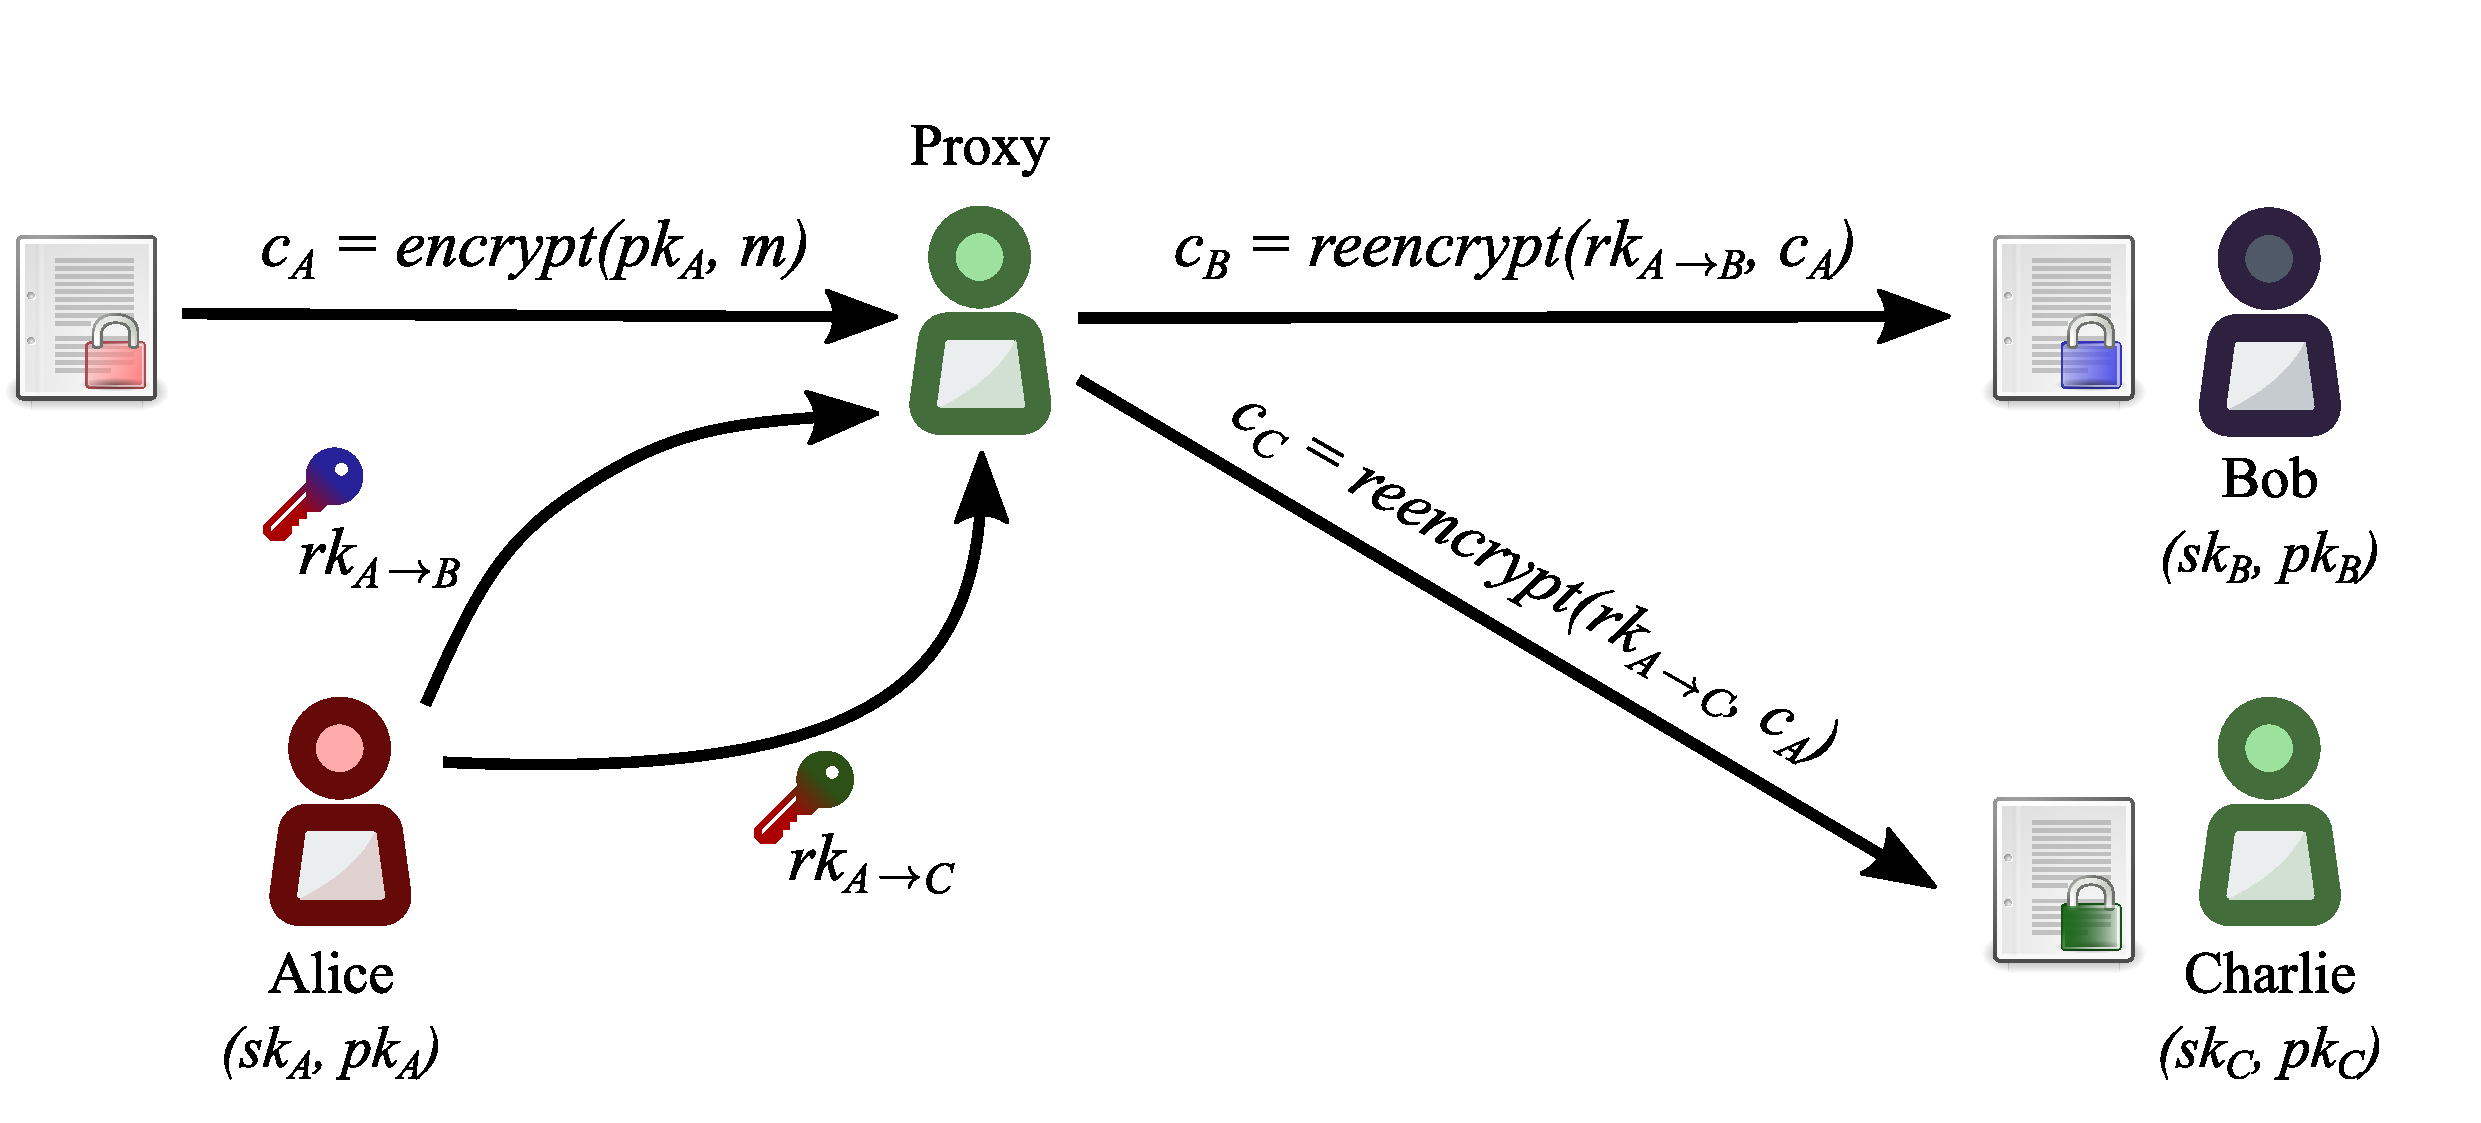
\includegraphics[width=13cm]{pdf/pre-multi.pdf}
        \end{figure}
    \end{frame}

    \begin{frame}
        \frametitle{Solution}
        \framesubtitle{Proxy re-encryption + Key Management}
        \begin{figure}
            \centering
            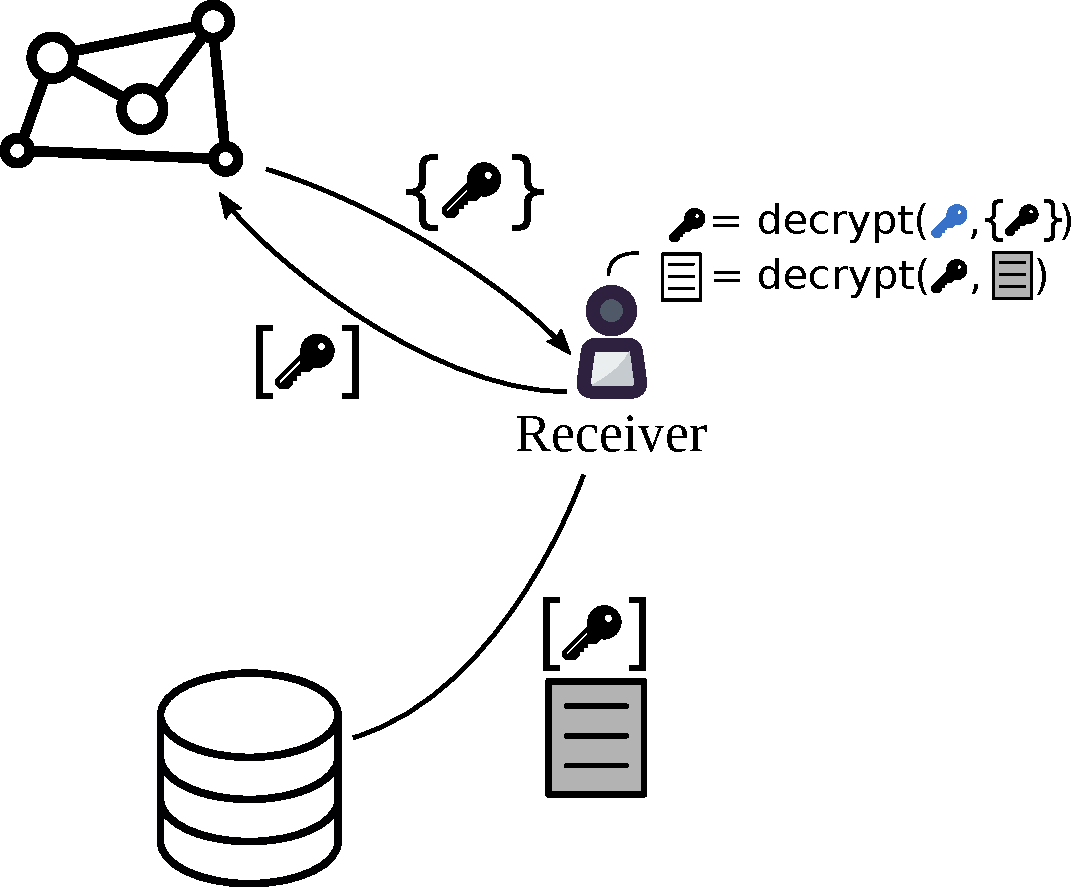
\includegraphics[height=6.5cm]{pdf/pre-kms.pdf}
        \end{figure}
    \end{frame}

    \begin{frame}
        \frametitle{Centralized KMS using PRE}
        \framesubtitle{Encryption}
        \begin{figure}
            \centering
            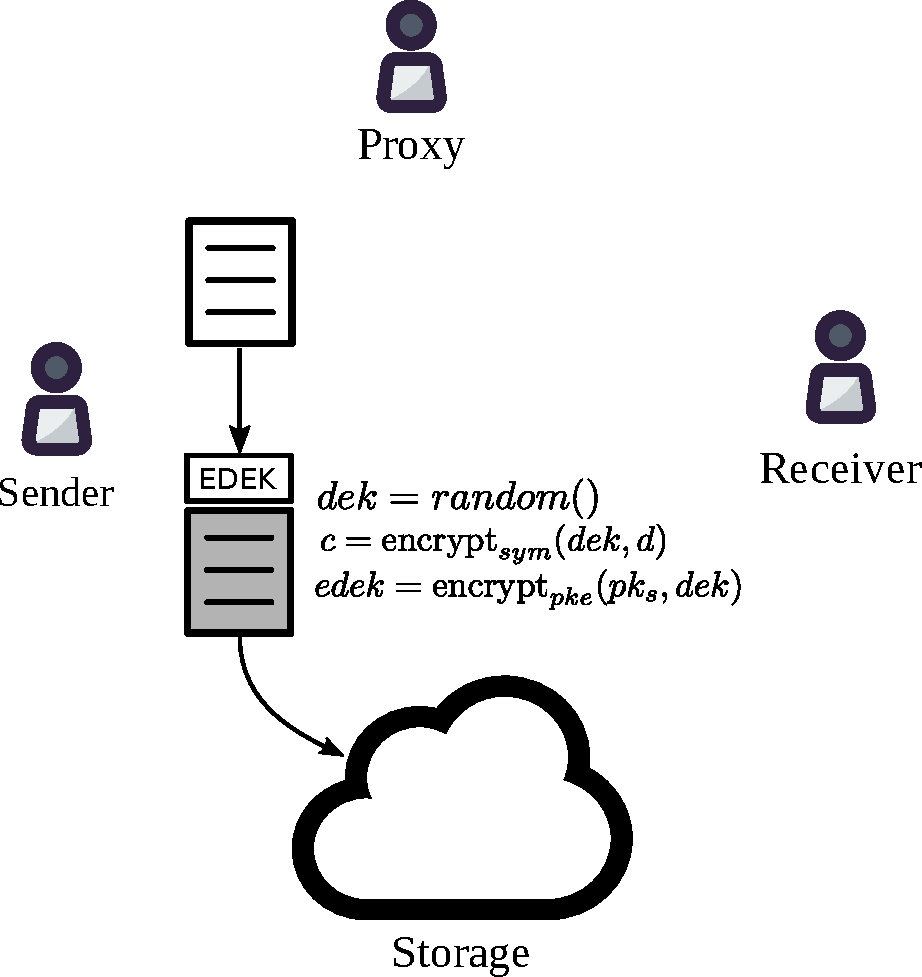
\includegraphics[height=7cm]{pdf/encrypt.pdf}
        \end{figure}
    \end{frame}

    \begin{frame}
        \frametitle{Centralized KMS using PRE}
        \framesubtitle{Access delegation}
        \begin{figure}
            \centering
            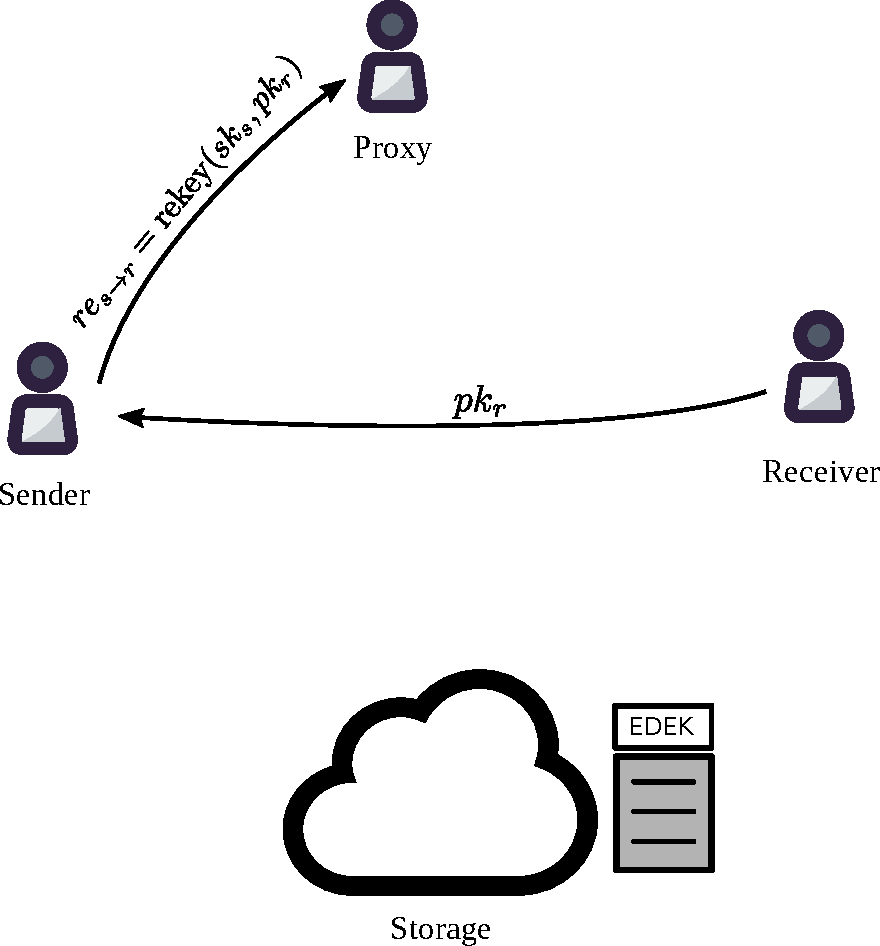
\includegraphics[height=7cm]{pdf/delegate.pdf}
        \end{figure}
    \end{frame}

    \begin{frame}
        \frametitle{Centralized KMS using PRE}
        \framesubtitle{Decryption}
        \begin{figure}
            \centering
            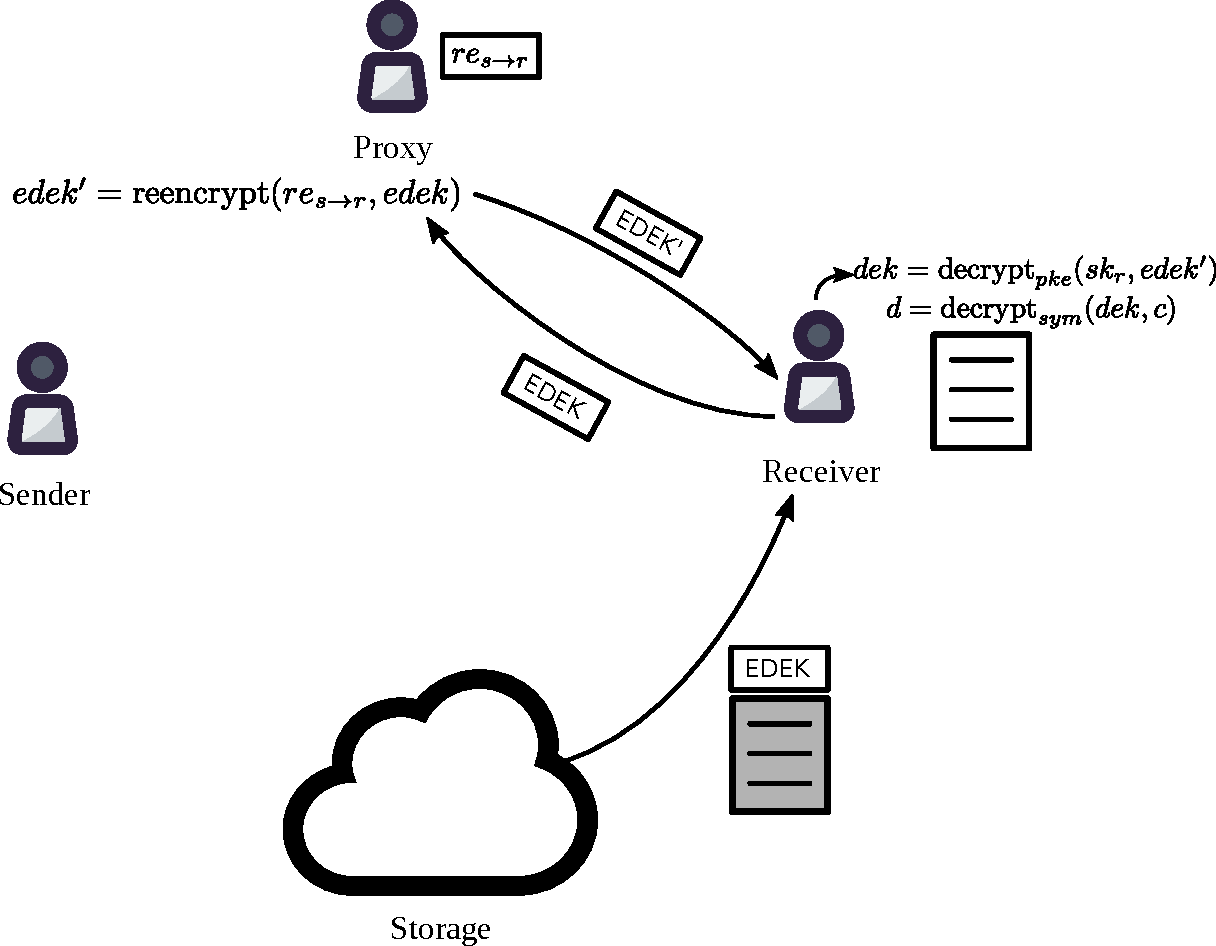
\includegraphics[height=7cm]{pdf/decrypt.pdf}
        \end{figure}
    \end{frame}

    \begin{frame}
        \frametitle{Decentralized Key Management}
        \framesubtitle{Using threshold split-key re-encryption (Umbral)}
        \begin{figure}
            \centering
            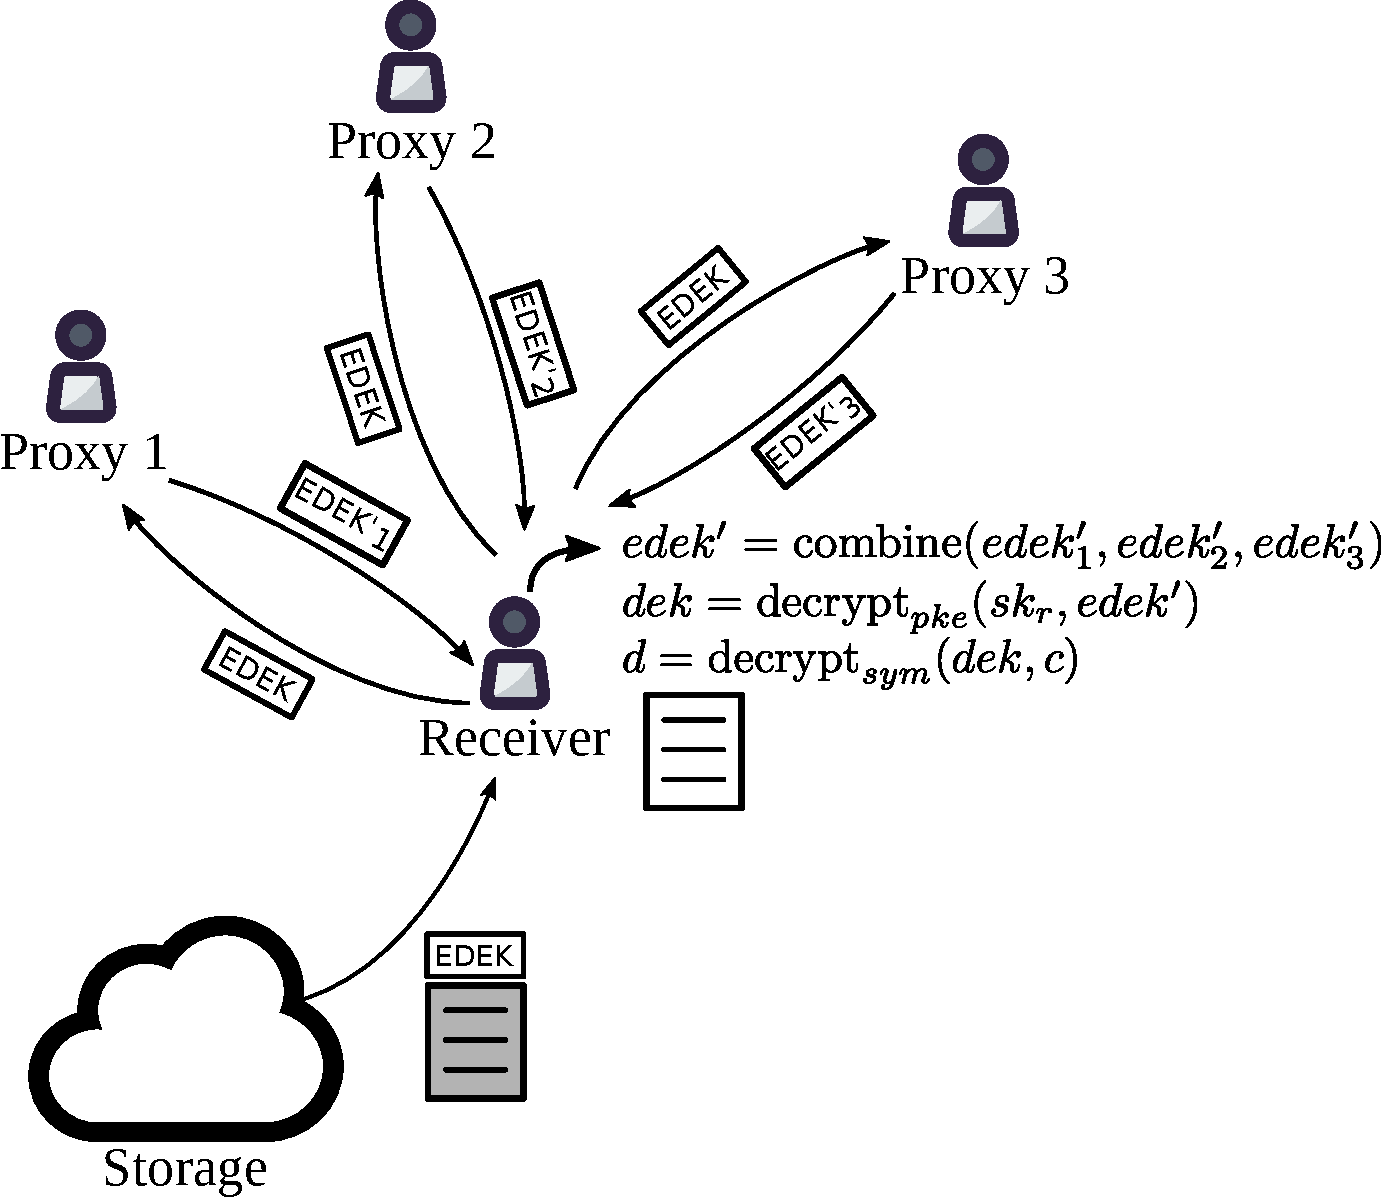
\includegraphics[height=6.5cm]{pdf/decrypt-umbral.pdf}
        \end{figure}
    \end{frame}

    \begin{frame}
        \frametitle{Umbral: Threshold Proxy Re-encryption}
        \begin{itemize}
        	\item \emph{``Umbral''} is Spanish for \emph{``threshold''}
            \item PRE properties: Unidirectional, single-hop, non-interactive
            \item It follows a KEM/DEM approach:
            	\begin{itemize}
		    \item UmbralKEM provides the threshold re-encryption capability
                    \item Uses ECIES for key encapsulation with zero knowledge proofs of correctness for verifiability on prime order curves (such as secp256k1)
            	    \item The DEM can be any authenticated encryption (currently ChaCha20-Poly1305)
        	\end{itemize}
	    \item IND-PRE-CCA security
            \item Key splitting is analogous to Shamir Secret Sharing
	    \item Verification of re-encryption correctness through Non-Interactive ZK Proofs
            \item Reference implementation: \url{https://github.com/nucypher/pyUmbral/}
	    \item Documentation (WIP): \url{https://github.com/nucypher/umbral-doc}
        \end{itemize}
    \end{frame}

    \begin{frame}
        \frametitle{KMS Network: Data Sharing + PKE}
        \begin{figure}
            \centering
            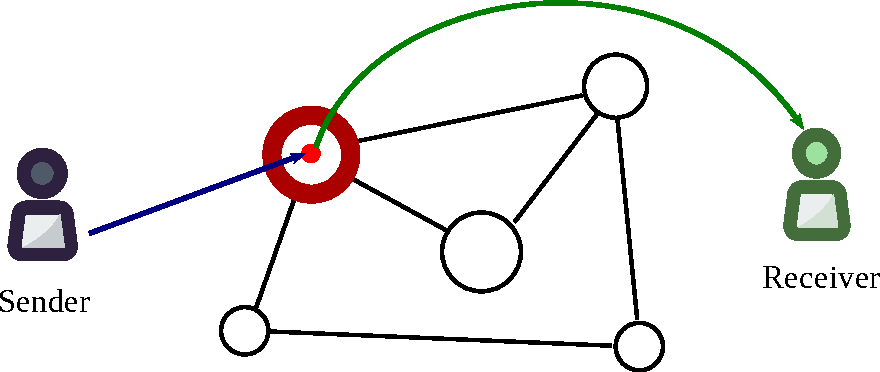
\includegraphics[height=5.5cm]{pdf/permissioned.pdf}
        \end{figure}
        \begin{itemize}
            \item Single node has access to data
            \item Single node can deny to do work
        \end{itemize}
    \end{frame}

    \begin{frame}
        \frametitle{KMS Network: Data Sharing + PKE + Shamir Secret Sharing}
        \begin{figure}
            \centering
            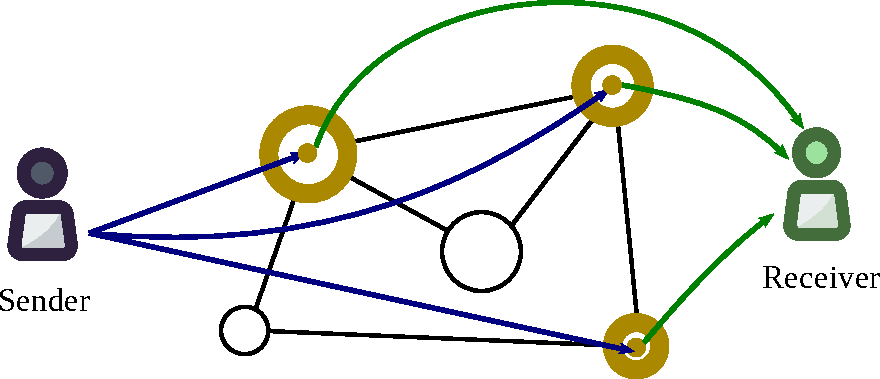
\includegraphics[height=5.5cm]{pdf/permissioned-sss.pdf}
        \end{figure}
        \begin{itemize}
            \item Nodes can collude to gain access to data
        \end{itemize}
    \end{frame}

    \begin{frame}
        \frametitle{KMS Network: Data Sharing + PRE}
        \begin{figure}
            \centering
            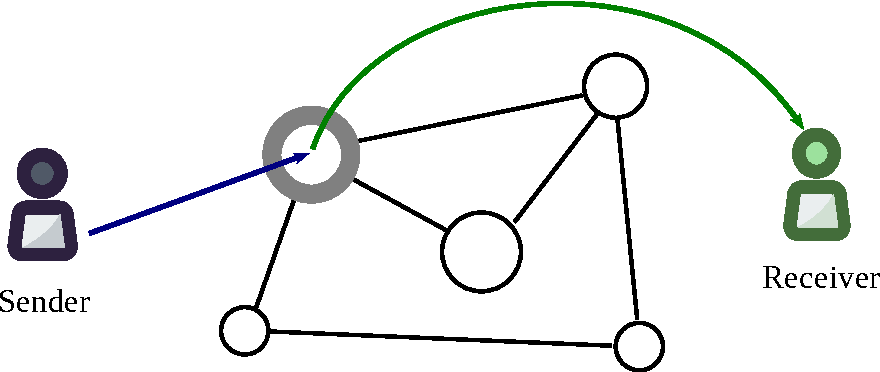
\includegraphics[height=5.5cm]{pdf/prenodes.pdf}
        \end{figure}
        \begin{itemize}
            \item Single node collusion with receiver possible
            \item Single node can deny to do work.
        \end{itemize}
    \end{frame}

    \begin{frame}
        \frametitle{KMS Network: Data Sharing + Threshold PRE (Umbral)}
        \begin{figure}
            \centering
            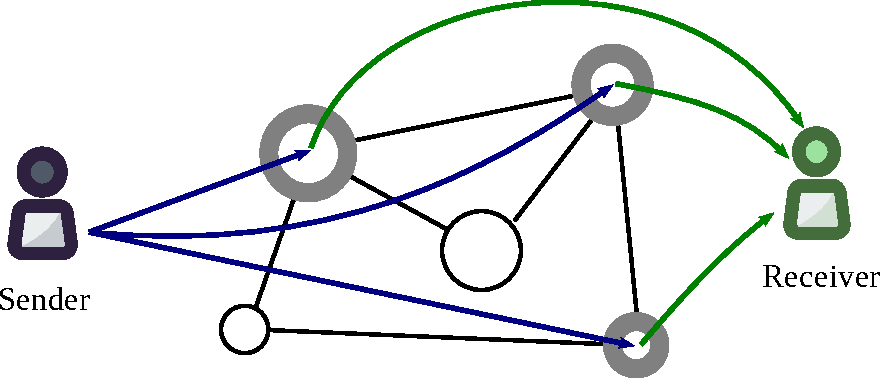
\includegraphics[height=5.5cm]{pdf/umbralnodes.pdf}
        \end{figure}
        \begin{itemize}
            \item Collusion now requires $m$ nodes + receiver
        \end{itemize}
    \end{frame}

    \begin{frame}
        \frametitle{NU Token}
        \framesubtitle{Purpose}
        \begin{itemize}
            \item Splitting trust across re-encryption nodes: more tokens = more trust and more work
            \item Proof of Stake for minting new coins according to the mining schedule
            \item Security deposit at stake against malicious behavior of nodes
        \end{itemize}
    \end{frame}

   \begin{frame}
        \frametitle{Data Sharing Policies}
        \begin{itemize}
            \item Time-based
            \item Conditional on payment 
            \begin{itemize}
              \item ``grant access once paid, continue granting while paying''
            \end{itemize}
            \item Smart contract (public) method
        \end{itemize}
        Decentralized re-encryption nodes (Ursulas) are trusted to apply conditions without decrypting data
    \end{frame}

    \begin{frame}
        \frametitle{Demo}
        \begin{figure}
            \centering
            
\includegraphics[height=5.5cm]{pdf/terminal.pdf}
        \end{figure}
    \end{frame}

    \begin{frame}
        \frametitle{Use Cases}
        \framesubtitle{Encrypted file sharing}
        \begin{figure}
            \centering
            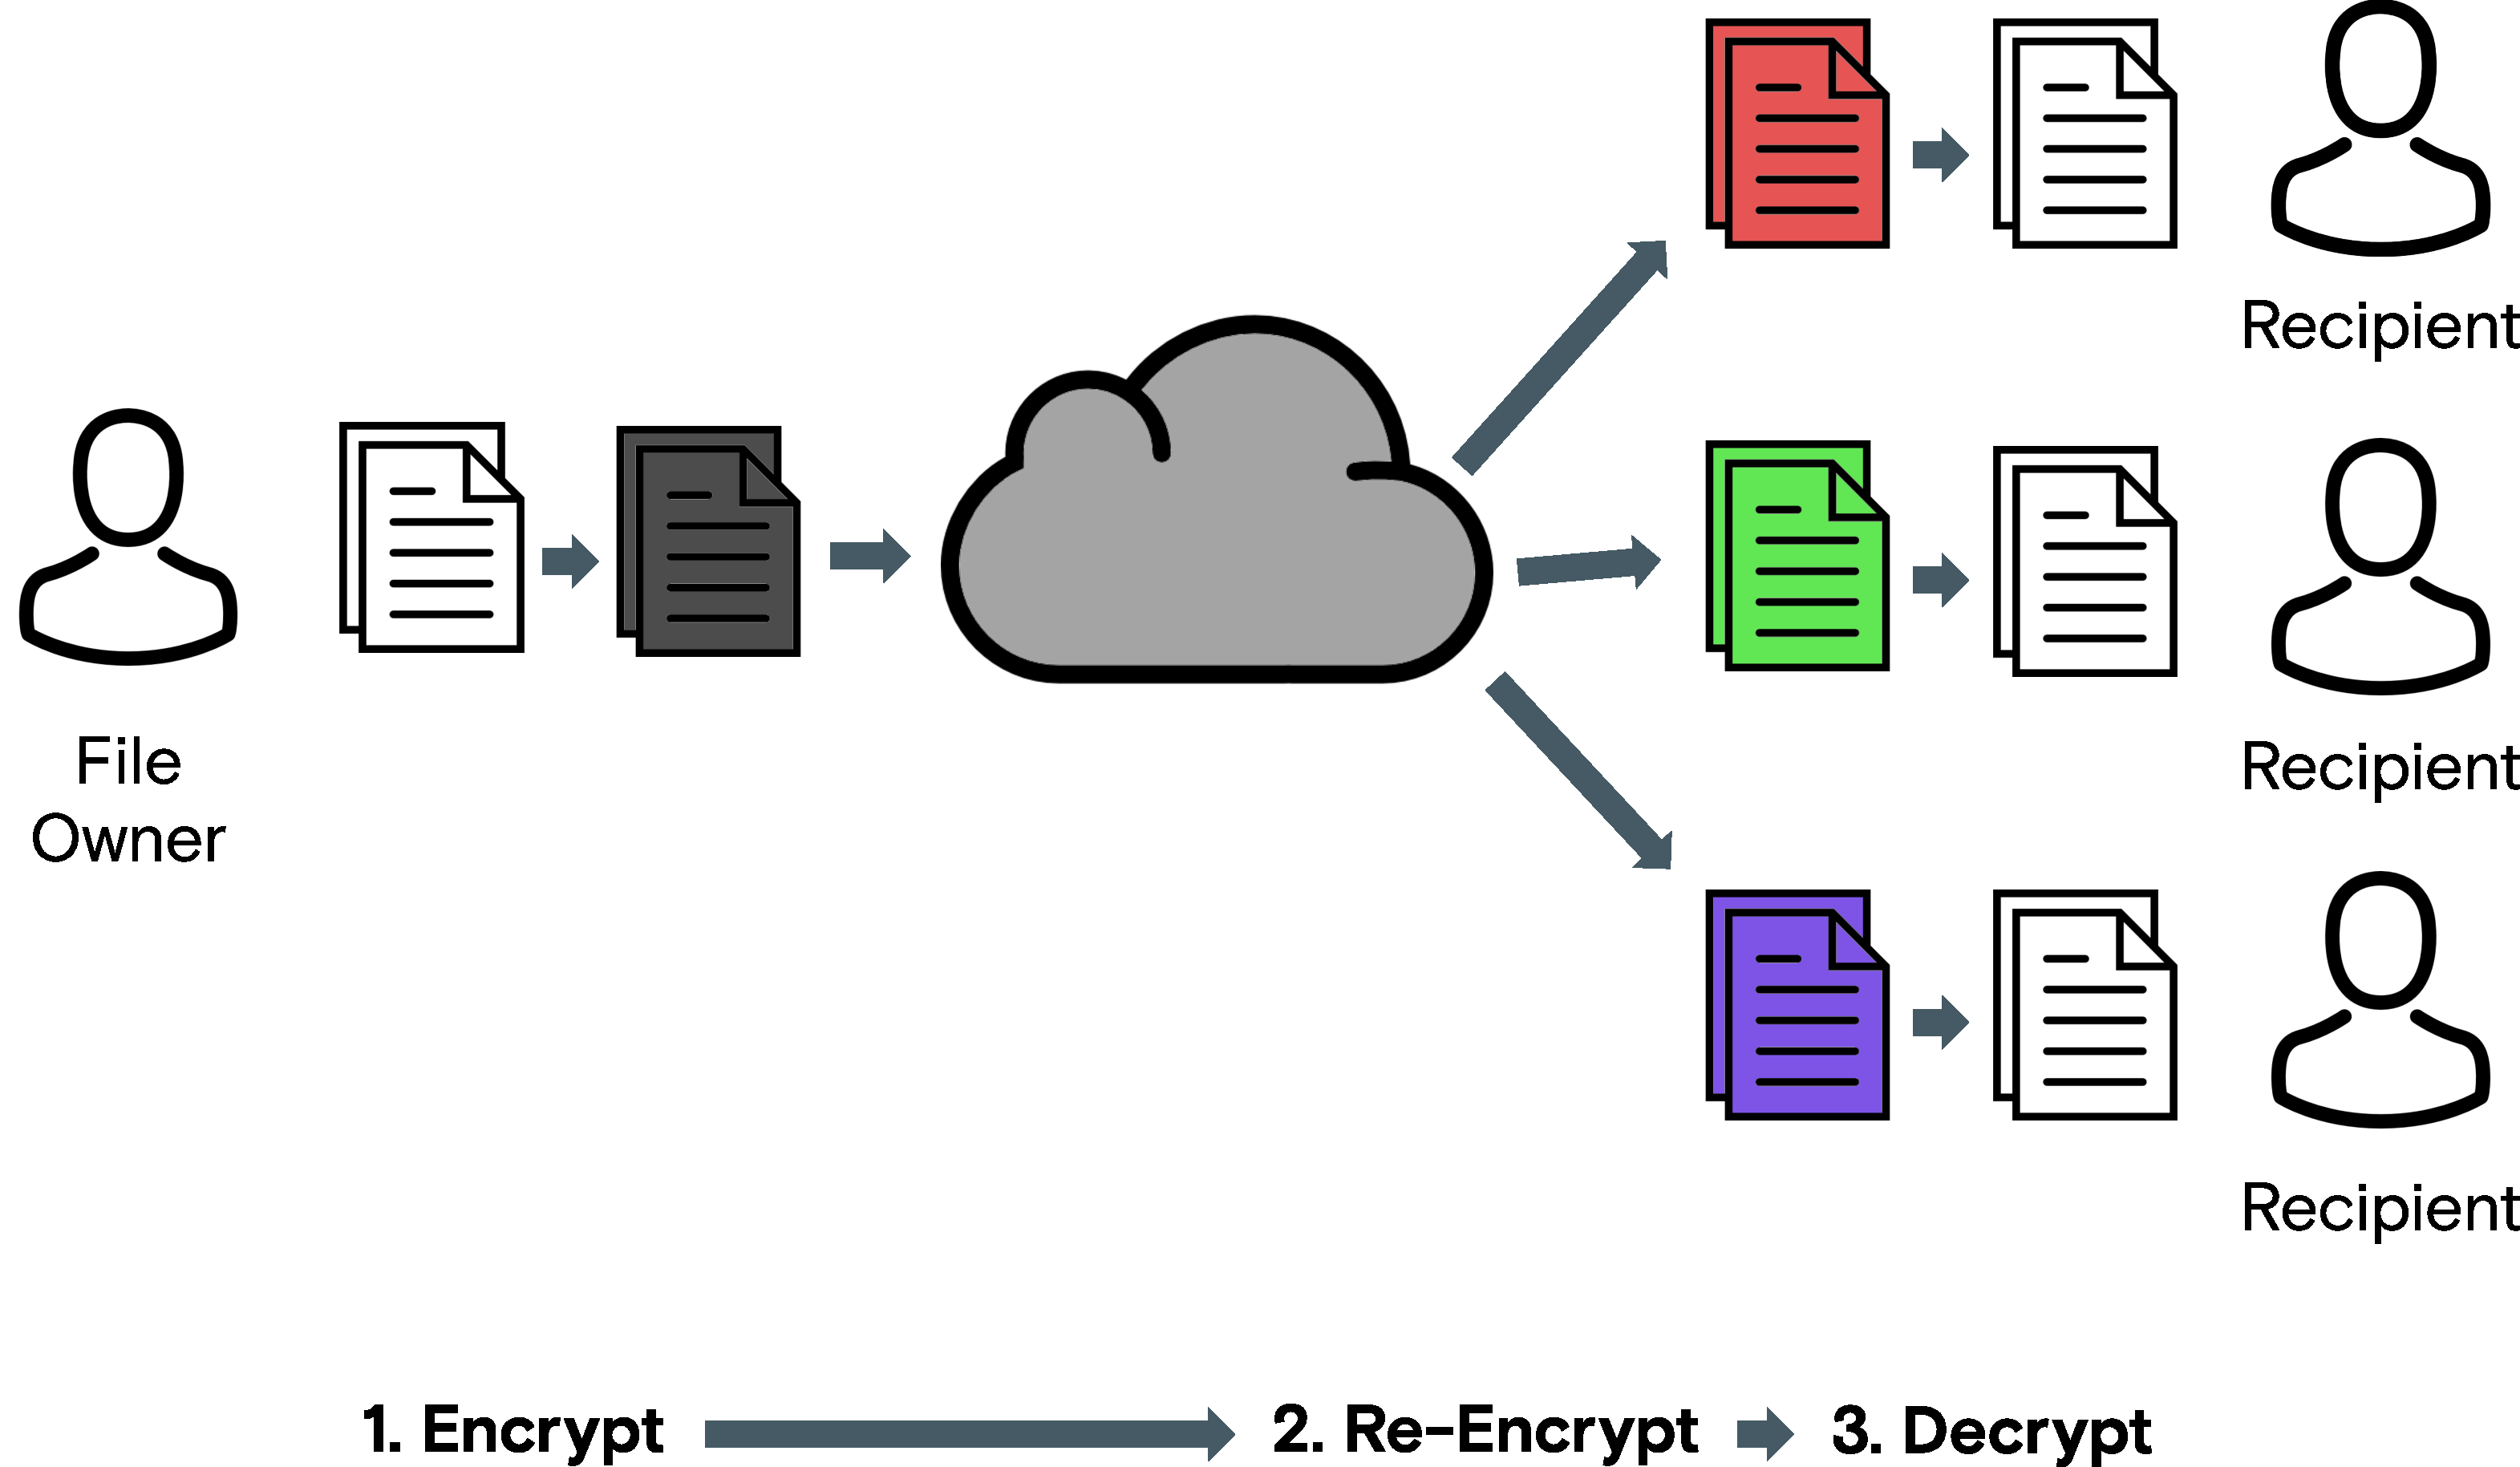
\includegraphics[height=7cm]{pdf/file-sharing-alternative.pdf}
        \end{figure}
    \end{frame}

    \begin{frame}
        \frametitle{Use Cases}
        \framesubtitle{Encrypted multi-user chats}
        \begin{figure}
            \centering
            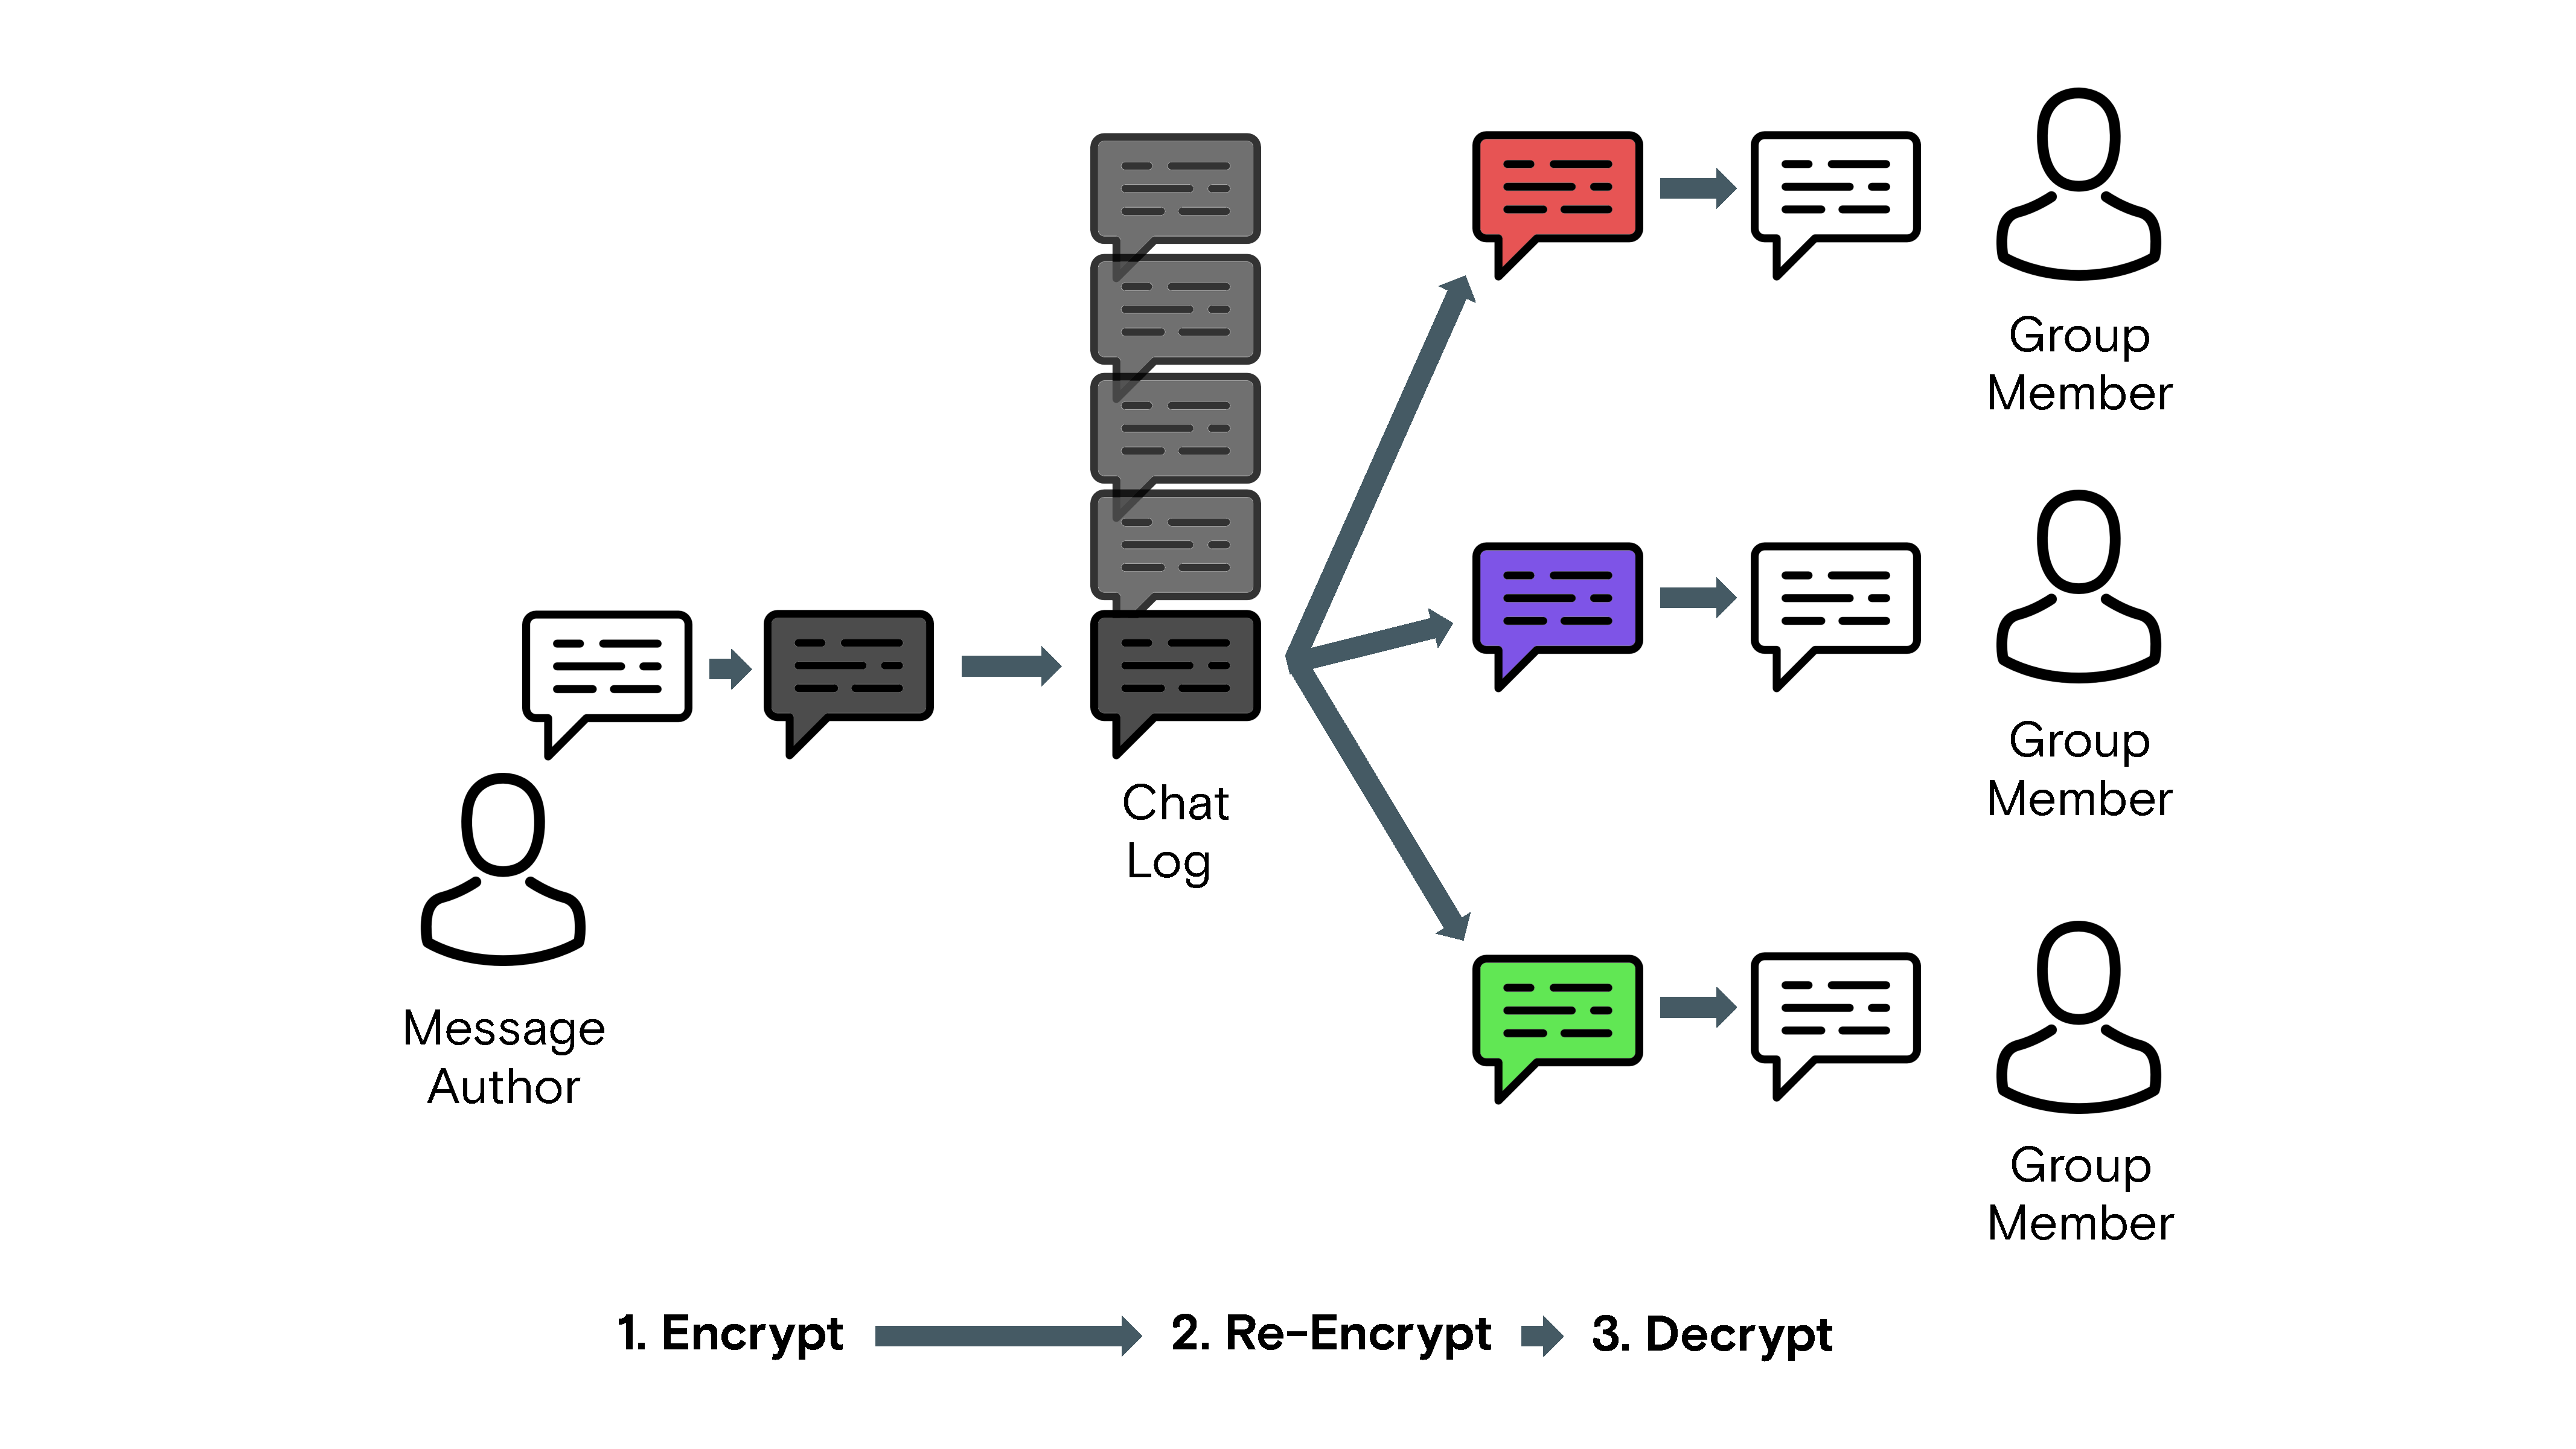
\includegraphics[height=7cm]{pdf/chats-alternative.pdf}
        \end{figure}
    \end{frame}

    \begin{frame}
        \frametitle{Use Cases}
        \framesubtitle{Decentralized Access-Controlled Content}
        \begin{figure}
            \centering
            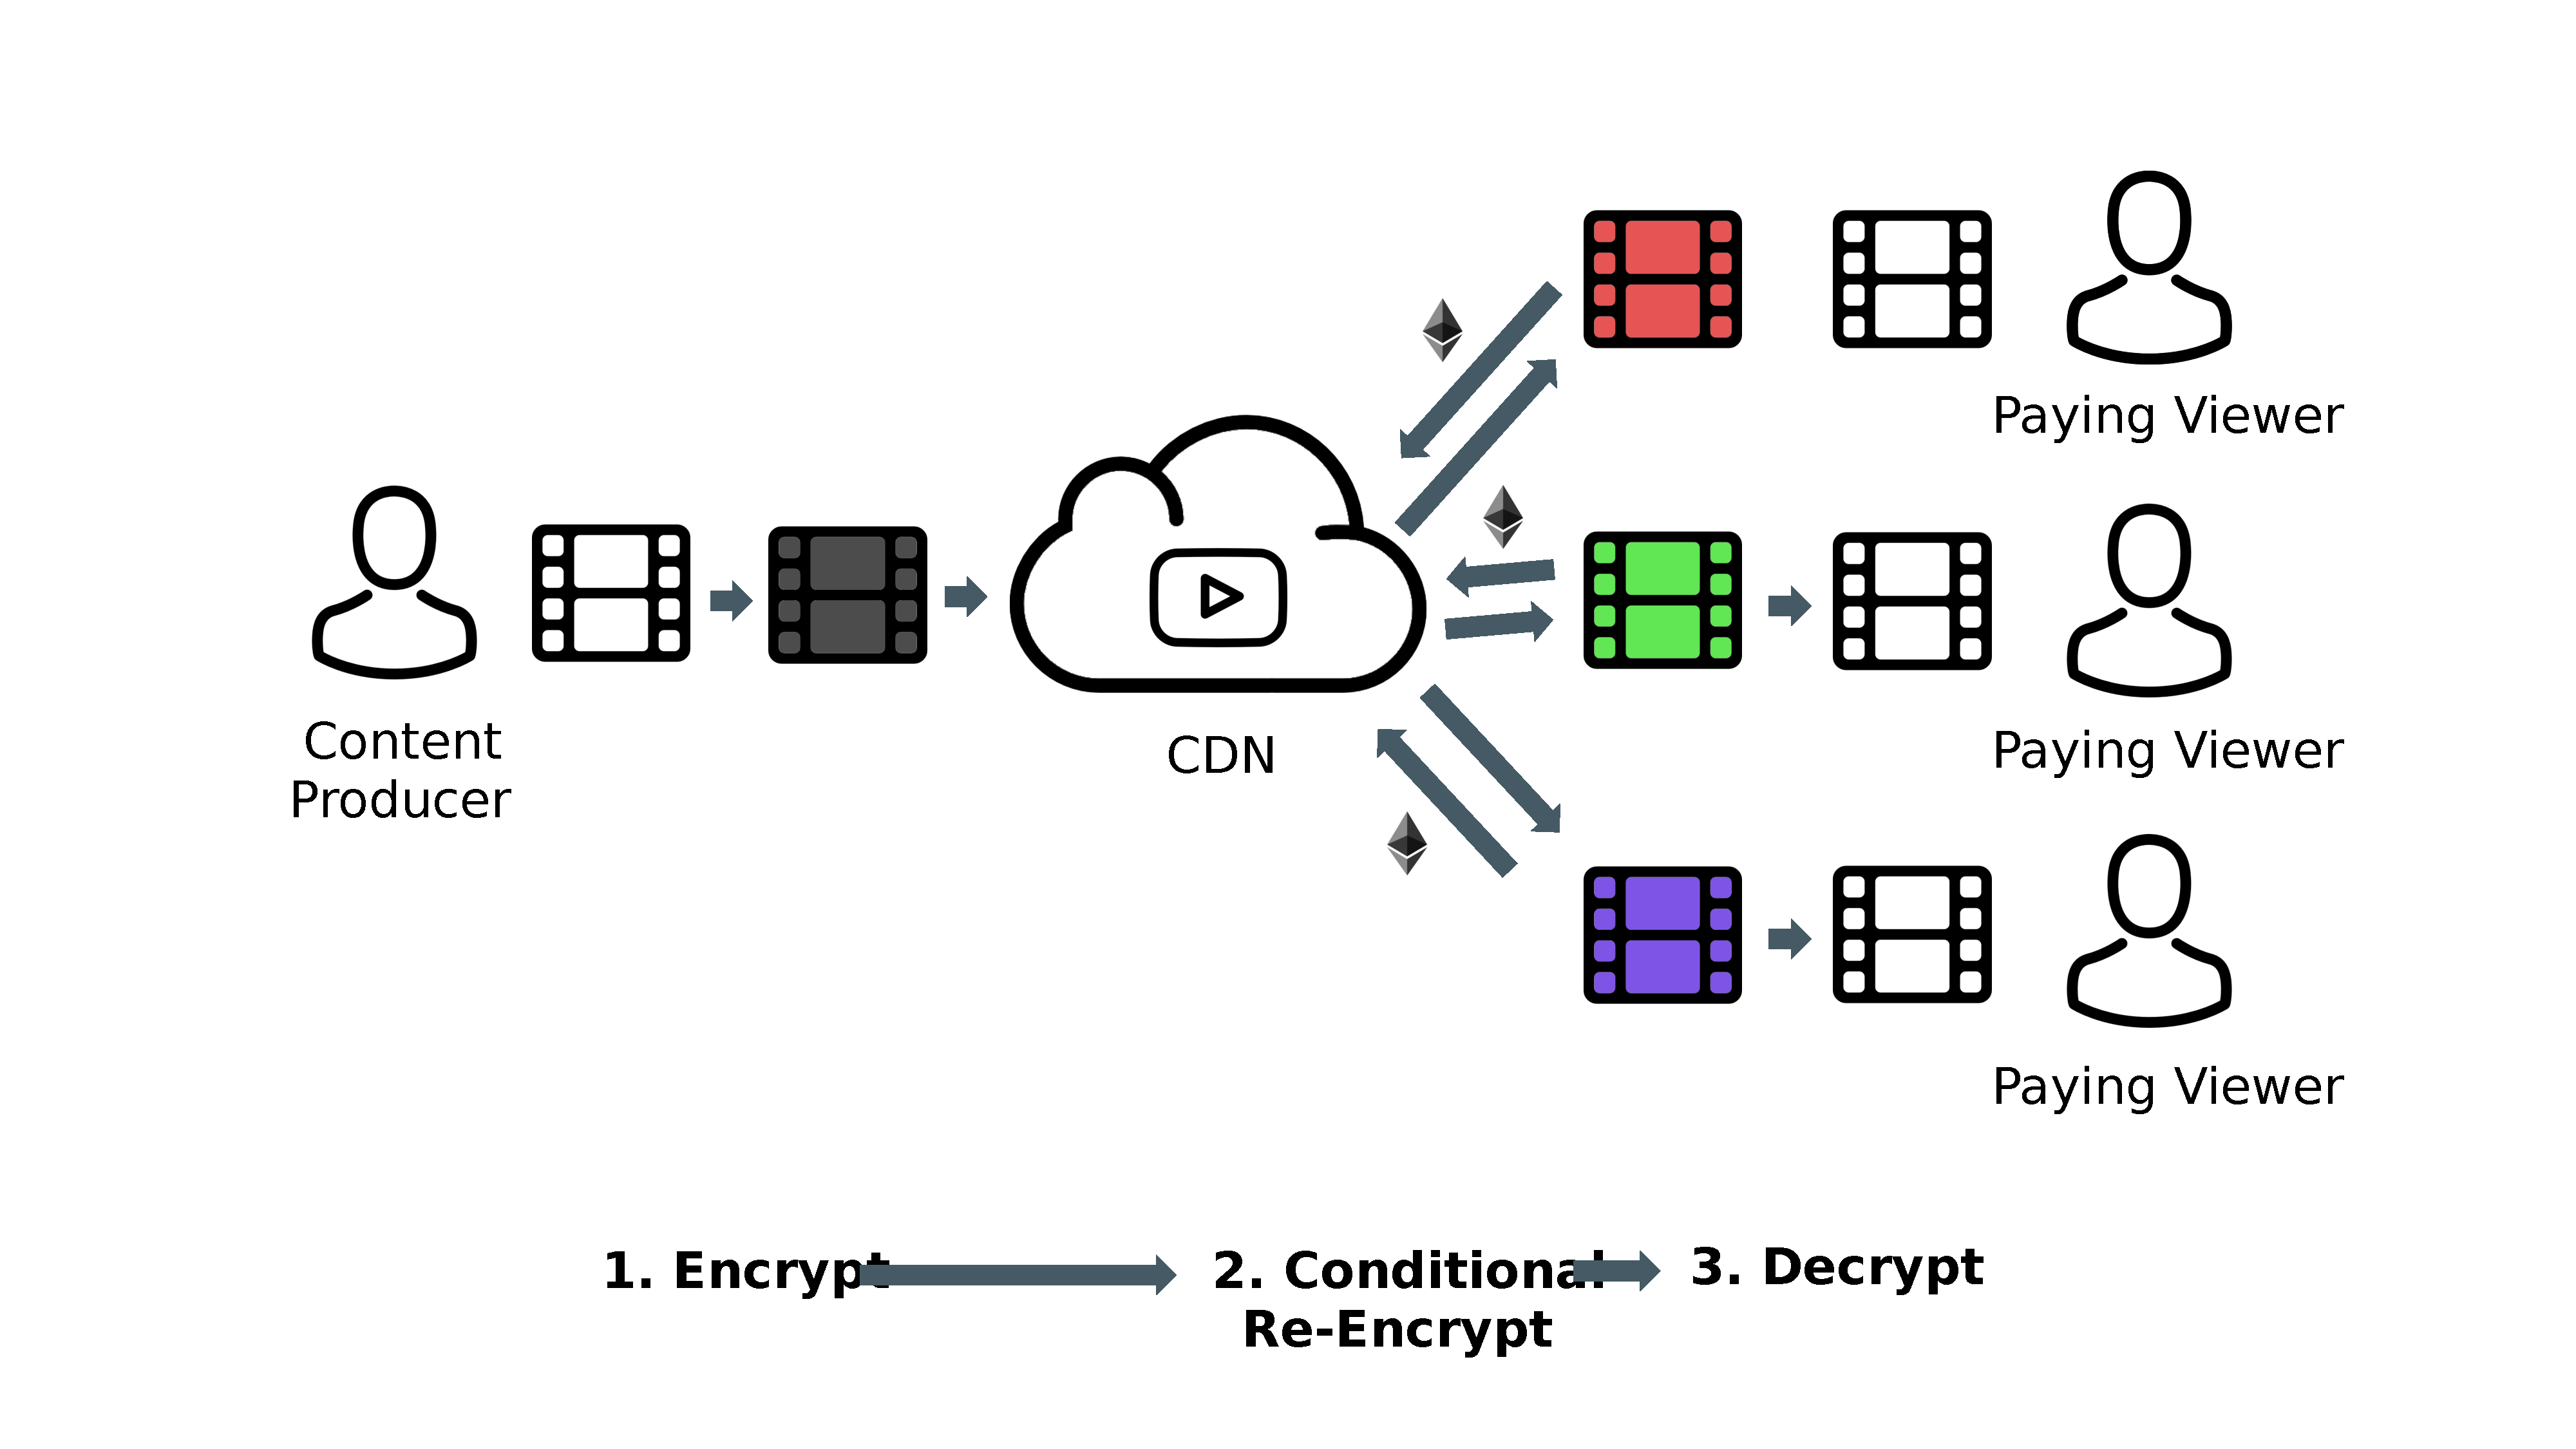
\includegraphics[height=7cm]{pdf/streams-alternative.pdf}
        \end{figure}
    \end{frame}

    \begin{frame}
      \frametitle{Early Users}
      \begin{figure}
           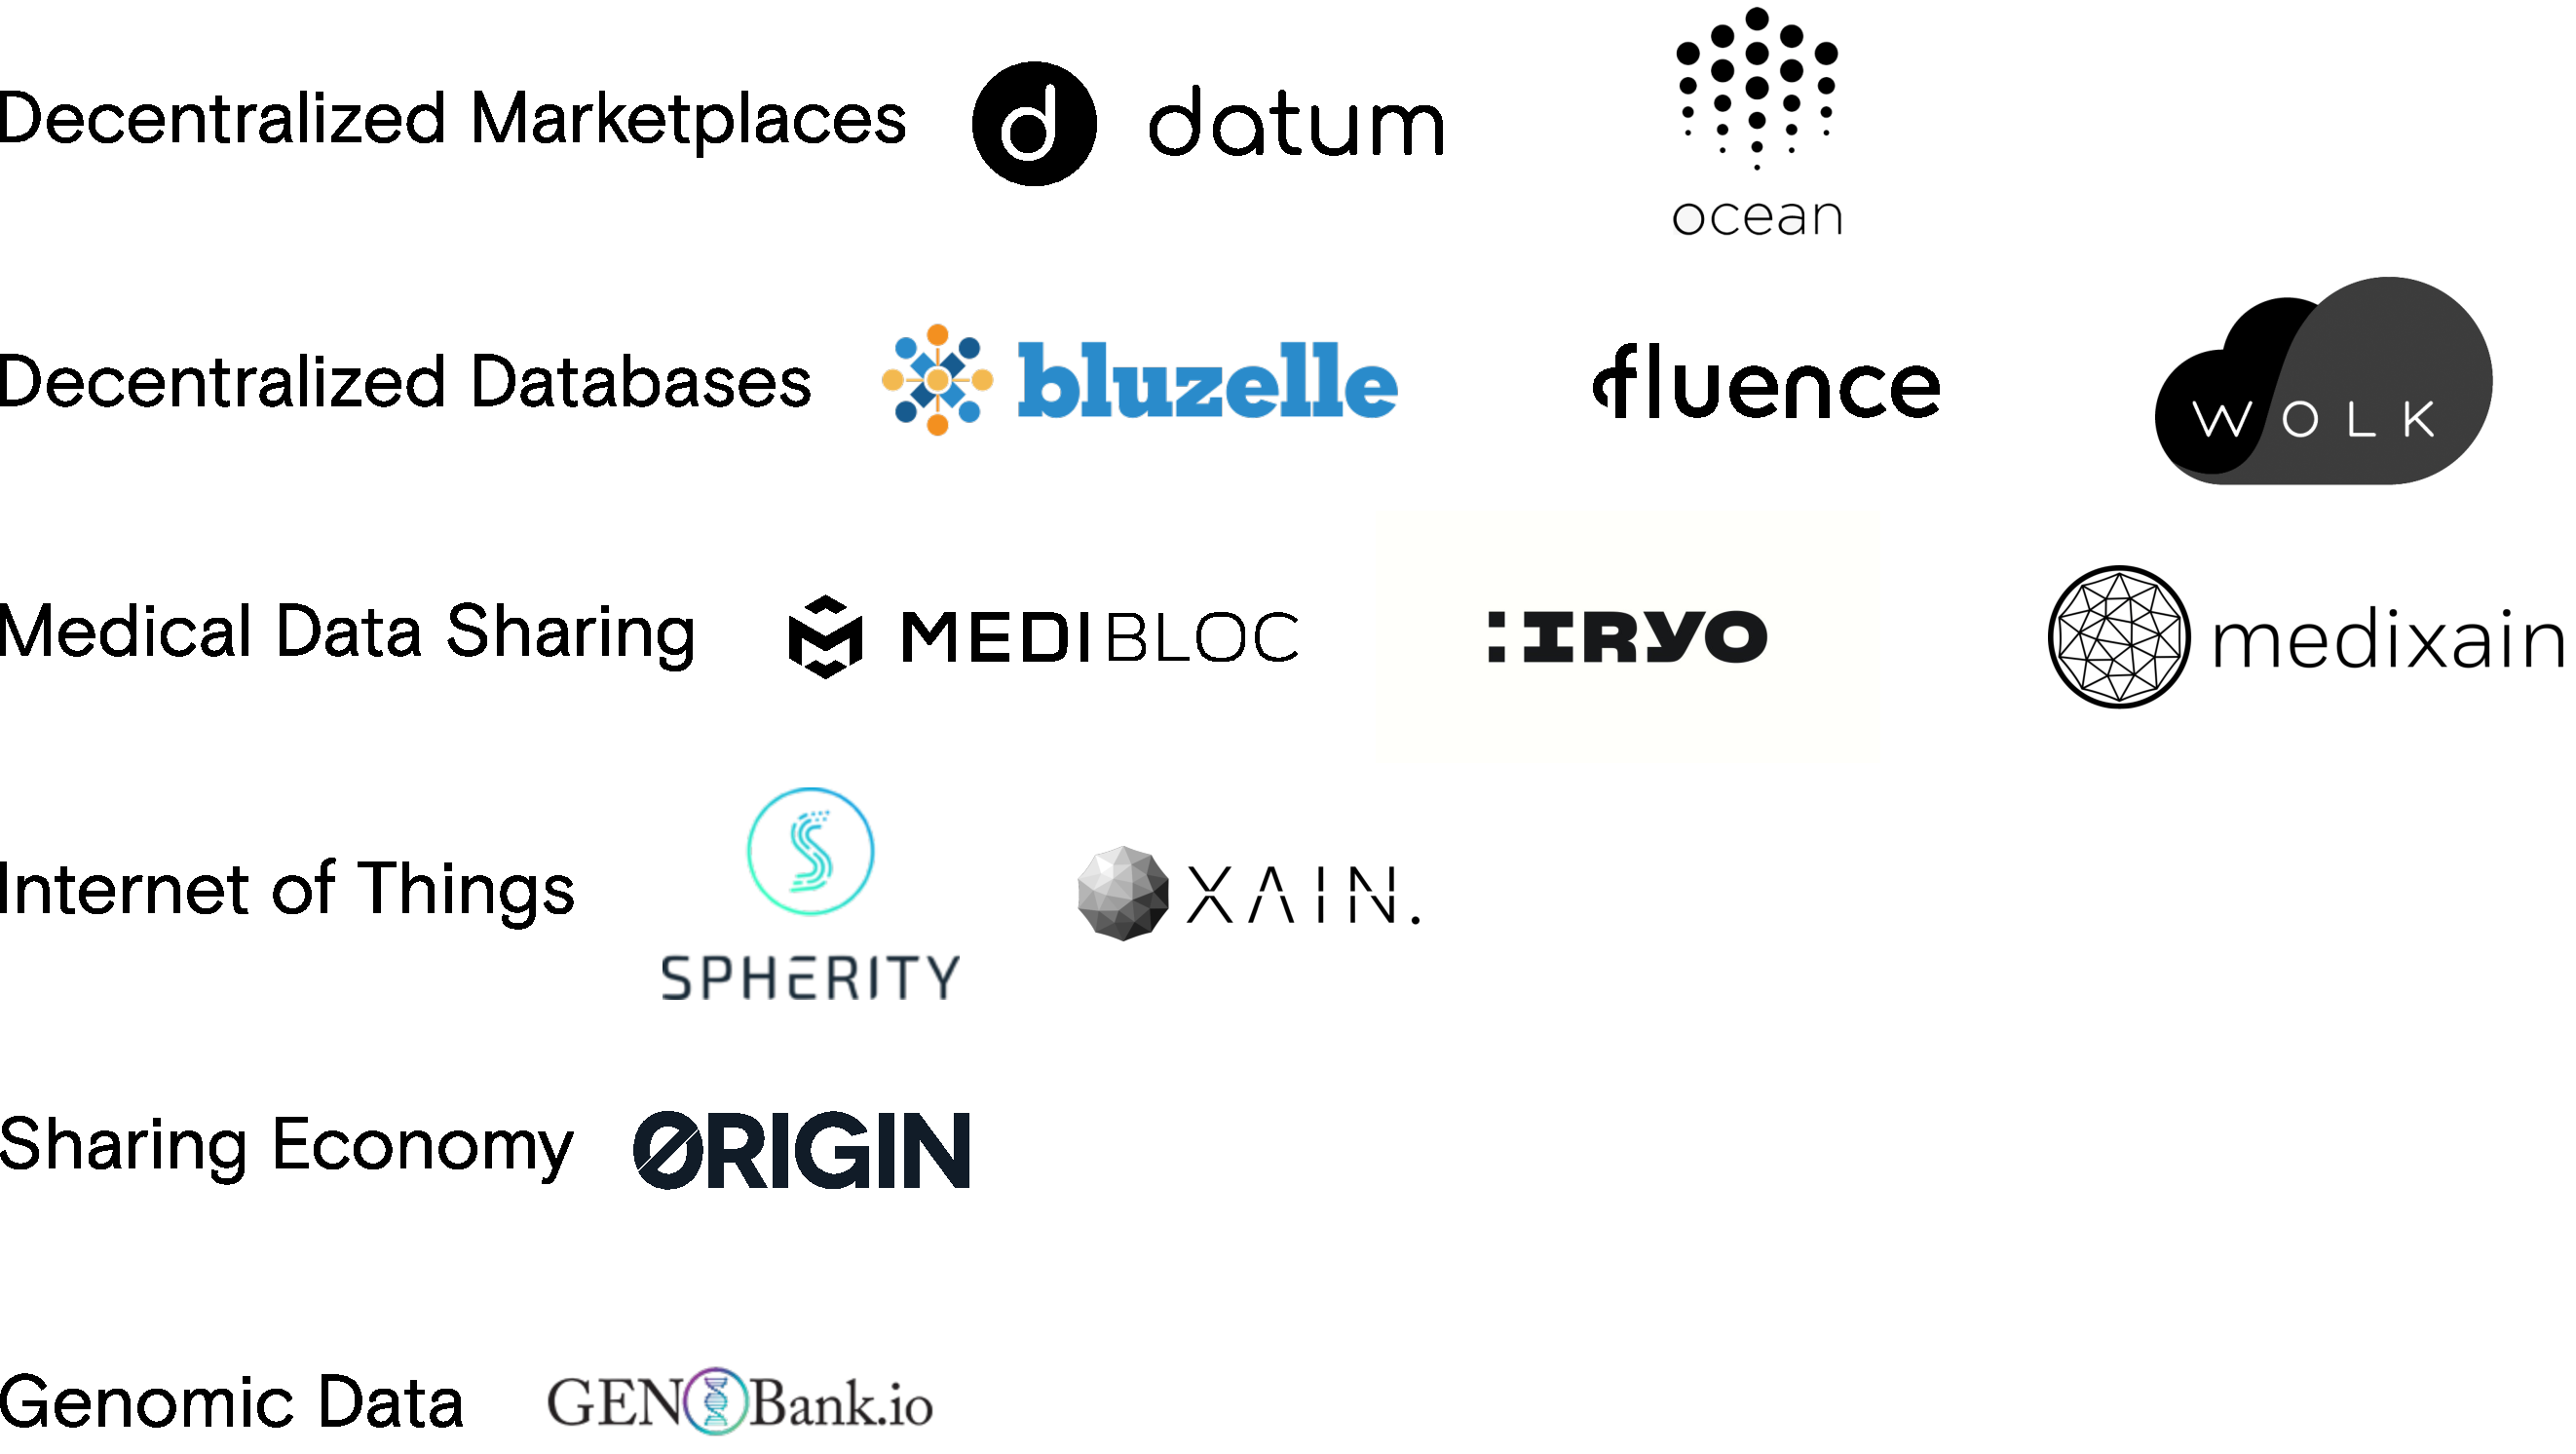
\includegraphics[width=11.5cm]{pdf/projects.pdf}
      \end{figure}
    \end{frame}

    \begin{frame}
      \frametitle{Competing Technology}
       Data Masking and Tokenization
       \begin{itemize}
           \item Less secure for data with underlying patterns
           \item Reduce the value of data by obfuscating it
       \end{itemize}

       Public Key Encryption
       \begin{itemize}
           \item Data must be decrypted before it is shared
           \item Not Scalable
       \end{itemize}

       Multi-Party Computation
       \begin{itemize}
           \item Interactive protocol
           \item Slow Performance
       \end{itemize}

       Fully Homomorphic Encryption
       \begin{itemize}
           \item Slow Peformance
           \begin{itemize}
               \item NuCypher is investing efforts in this area
           \end{itemize}
       \end{itemize}
     \end{frame}

    \begin{frame}
      \frametitle{Fully Homomorphic Encryption}
       \framesubtitle{nuFHE Library}
       \begin{itemize}
           \item GitHub: \url{https://github.com/nucypher/nufhe}
           \item GPU implementation of fully homomorphic encryption
           \item Uses either FFT or integer NTT
           \item Achieved 100x performance over TFHE benchmarks
           \begin{figure}
               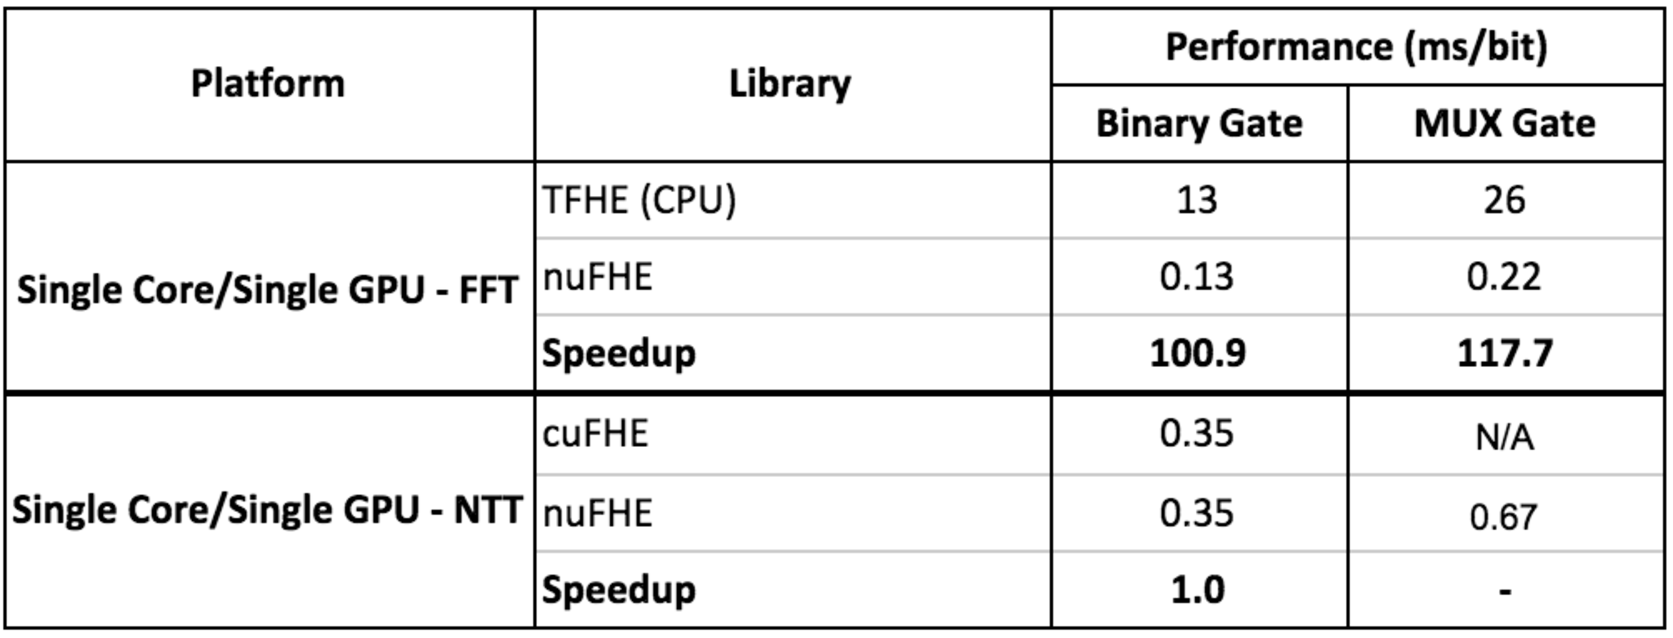
\includegraphics[width=10.5cm]{pdf/nufhe-benchmarks.pdf}
           \end{figure}
       \end{itemize}
     \end{frame}

    \begin{frame}
        \frametitle{More Information}
        \begin{figure}
            \centering
            
\includegraphics[width=3cm]{pdf/nucypher_logo.pdf}
        \end{figure}
        Website: \url{https://nucypher.com}

        Github: \url{https://github.com/nucypher/}

        PyUmbral: \url{https://github.com/nucypher/pyUmbral/}

        GoUmbral: \url{https://github.com/nucypher/goUmbral/}

        Mocknet: \url{https://github.com/nucypher/mock-net/}

        Discord: \url{https://discord.gg/7rmXa3S}

        Whitepaper: \url{https://www.nucypher.com/whitepapers/english.pdf}

        E-mail: \href{mailto:\emailname @nucypher.com}{\emailname @nucypher.com}

        E-mail: \href{mailto:hello@nucypher.com}{hello@nucypher.com}
    \end{frame}

    \begin{frame}
      \frametitle{Appendix: Umbral Flow Diagram}
      \begin{figure}
        \centering
        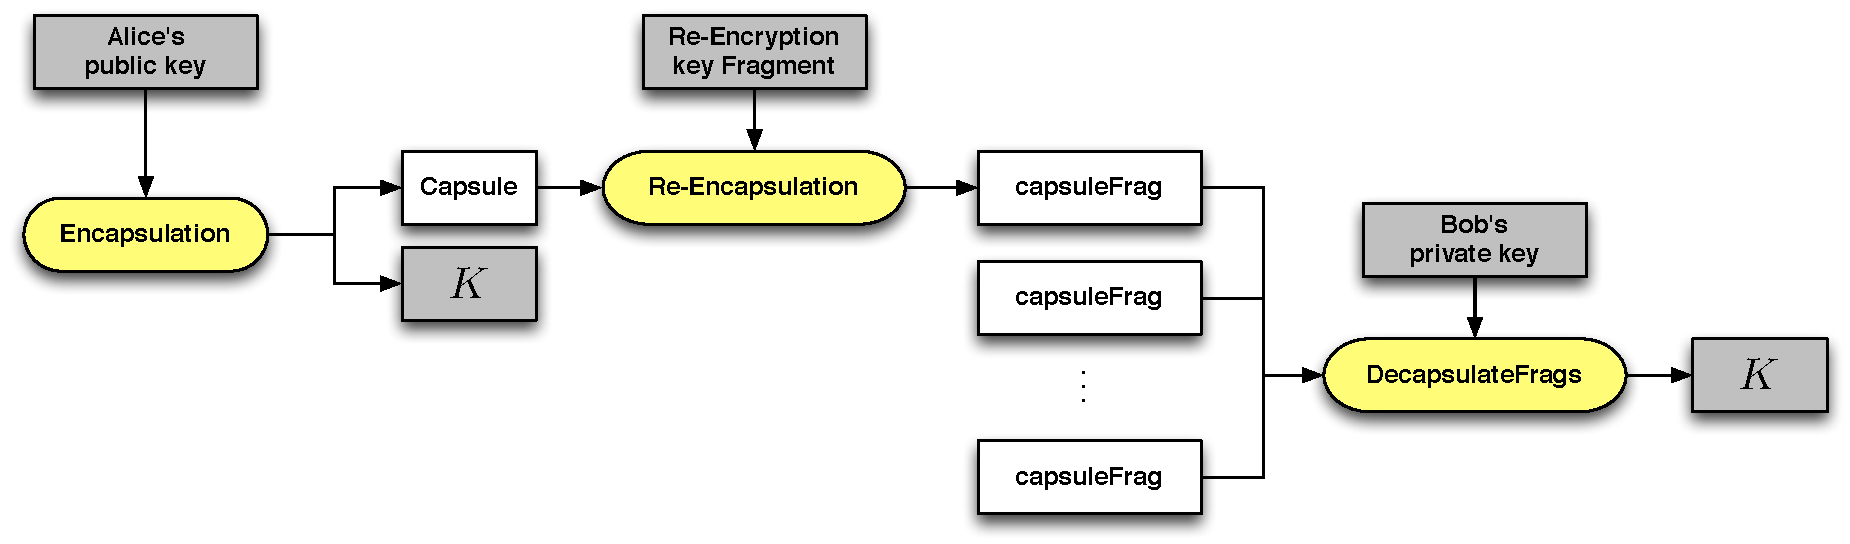
\includegraphics[width=11cm]{pdf/umbral-kem-flow.pdf}
      \end{figure}
      \begin{itemize}
           \item Reference implementation: \url{https://github.com/nucypher/pyUmbral/}
           \item Documentation: \url{https://github.com/nucypher/umbral-doc}
      \end{itemize}
    \end{frame}

    \begin{frame}
        \frametitle{Appendix: Security Audits}
        \begin{figure}
            \centering
            
\includegraphics[height=2.5cm]{pdf/security-audits.pdf}
      \end{figure}
    \end{frame}

    \begin{frame}
        \frametitle{Appendix: NU Token Metrics}
        \framesubtitle{Mining}
        Mining reward:
        \begin{eqnarray}
            \kappa &=& \left(0.5 + 0.5\frac{\min(T_i, T_1)}{T_1}\right)\\
            T_{i,\text{initial}} &\ge& T_{\min},\\
            \delta s_{i,t} &=&  \kappa\, \frac{l_i}{\sum l_j} \frac{\ln{2}}{T_{1/2}} \left( S_{\max} - S_{t-1}\right).\\
        \end{eqnarray}
        Results into:
        $$\text{reward} \propto 2^{\frac{t}{T_{1/2}}}$$
    \end{frame}

    \begin{frame}
        \frametitle{Appendix: NU Token Metrics}
        \framesubtitle{Graph of daily mining compensation}
        \begin{figure}
            \centering
            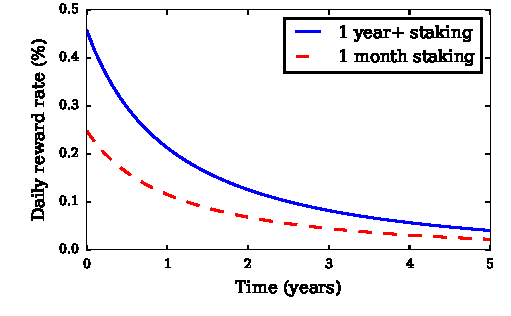
\includegraphics[height=5.5cm]{pdf/daily-compensation.pdf}
        \end{figure}
    \end{frame}

    \begin{frame}
        \frametitle{Appendix: NU Token Metrics}
        \framesubtitle{Relocking mining rewards}
        \begin{figure}
            \centering
            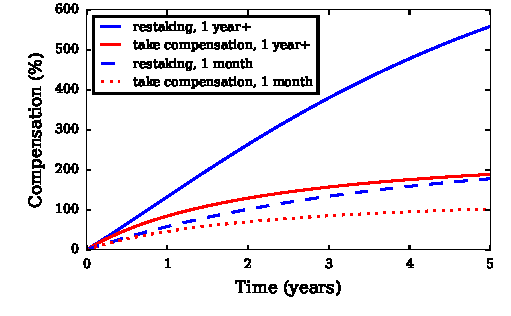
\includegraphics[height=5.5cm]{pdf/total-compensation.pdf}
        \end{figure}
    \end{frame}

    \begin{frame}
      \frametitle{Appendix: Team}
        \begin{figure}
            \centering
            \includegraphics[width=15cm]{pdf/company.pdf}
        \end{figure}
    \end{frame}

\end{document}

